\documentclass[border=3pt]{standalone}
\usepackage{fontspec}
\usepackage{unicode-math}
\setmainfont{texgyretermes}[Extension=.otf, UprightFont=*-regular, BoldFont=*-bold,
  ItalicFont=*-italic, BoldItalicFont=*-bolditalic]
\setsansfont{texgyreheros}[Extension=.otf, UprightFont=*-regular, BoldFont=*-bold]
\setmathfont{texgyretermes-math.otf}
\newfontfamily\chessfont{Apple Symbols}
\usepackage{tikz}
\usepackage{pgfplots}
\pgfplotsset{compat=1.17}
\definecolor{light}{HTML}{EDEDED}
\definecolor{dark}{HTML}{7389B8}
\definecolor{edge}{HTML}{4A4A4A}
\definecolor{blue2}{HTML}{B9C6E0}
\begin{document}
\fontsize{8}{9.6}\selectfont
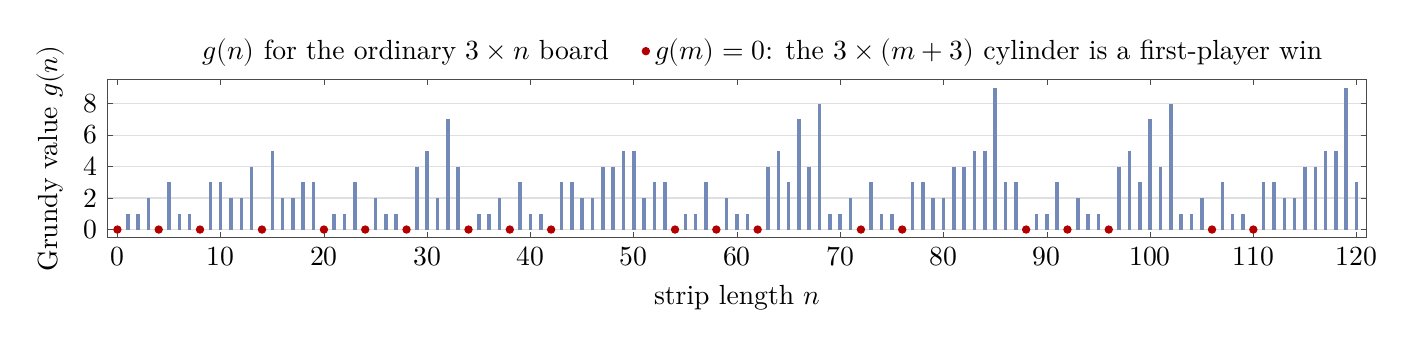
\begin{tikzpicture}\begin{axis}[scale only axis, width=16.0cm, height=2.0cm, xmin=-1, xmax=121,
  ymin=-0.5, ymax=9.5, xlabel={strip length $n$}, ylabel={Grundy value $g(n)$}, ytick={0,2,...,8},
  xtick={0,10,...,120}, ymajorgrids, grid style={gray!25}, axis line style={edge}, tick style={edge},
  major tick length=2pt,
  legend style={at={(0.5,1.03)}, anchor=south, legend columns=-1, draw=none,
    /tikz/every even column/.append style={column sep=10pt}}]
\addplot[ycomb, dark, line width=1.3pt] coordinates {(0,0) (1,1) (2,1) (3,2) (4,0) (5,3) (6,1) (7,1) (8,0) (9,3) (10,3) (11,2) (12,2) (13,4) (14,0) (15,5) (16,2) (17,2) (18,3) (19,3) (20,0) (21,1) (22,1) (23,3) (24,0) (25,2) (26,1) (27,1) (28,0) (29,4) (30,5) (31,2) (32,7) (33,4) (34,0) (35,1) (36,1) (37,2) (38,0) (39,3) (40,1) (41,1) (42,0) (43,3) (44,3) (45,2) (46,2) (47,4) (48,4) (49,5) (50,5) (51,2) (52,3) (53,3) (54,0) (55,1) (56,1) (57,3) (58,0) (59,2) (60,1) (61,1) (62,0) (63,4) (64,5) (65,3) (66,7) (67,4) (68,8) (69,1) (70,1) (71,2) (72,0) (73,3) (74,1) (75,1) (76,0) (77,3) (78,3) (79,2) (80,2) (81,4) (82,4) (83,5) (84,5) (85,9) (86,3) (87,3) (88,0) (89,1) (90,1) (91,3) (92,0) (93,2) (94,1) (95,1) (96,0) (97,4) (98,5) (99,3) (100,7) (101,4) (102,8) (103,1) (104,1) (105,2) (106,0) (107,3) (108,1) (109,1) (110,0) (111,3) (112,3) (113,2) (114,2) (115,4) (116,4) (117,5) (118,5) (119,9) (120,3)};
\addlegendentry{$g(n)$ for the ordinary $3\times n$ board}
\addplot[only marks, mark=*, mark size=1.3pt, red!70!black] coordinates {(0,0) (4,0) (8,0) (14,0) (20,0) (24,0) (28,0) (34,0) (38,0) (42,0) (54,0) (58,0) (62,0) (72,0) (76,0) (88,0) (92,0) (96,0) (106,0) (110,0)};
\addlegendentry{$g(m)=0$: the $3\times(m+3)$ cylinder is a first-player win}
\end{axis}\end{tikzpicture}
\end{document}
